\documentclass[11pt]{beamer}
\usepackage[utf8]{inputenc}
\usepackage[T1]{fontenc}
\usepackage{lmodern}
\usepackage[english]{babel}
\usetheme{AnnArbor}
\begin{document}
	\author{A R Bathri Narayanan}
	\title{The Gaussian Beam}
	\subtitle{Presentation for\\Femtosecond and Attosecond Pulses (P-704)}
	%\logo{}
	\institute{UM DAE Centre for Excellence in Basic Sciences}
	\date{November 25, 2024}
	\subject{Femtosecond and Attosecond pulses}
	%\setbeamercovered{transparent}
	%\setbeamertemplate{navigation symbols}{}
	\begin{frame}[plain]
		\maketitle
	\end{frame}
	
	\begin{frame}
		\frametitle{Prelude}
		A paraxial wave is a plane wave travelling along the z direction ($e^{-ikz}$) with wavenumber $\frac{2\pi}{\lambda}$ for wavelength $\lambda$, modulated by a complex envelope A(\textbf{r}), being a slowly varying function of position.  The complex amplitude is 
		\[U(\textbf{r})=A(\textbf{r})e^{-ikz}\]
		The envelope is taken to be approximately constant within a
		neighborhood of size $\lambda$, so that the wave locally maintains its plane-
		wave nature but exhibits wavefront normals that are paraxial rays.\\
		In order that the complex amplitude U(\textbf{r}) satisfy the Helmholtz
		equation, $\nabla^2U+k^2U=0$. The paraxial envelope should ba a solution of the Paraxial Helmholtz equation
		\[\nabla^2_T A -j2k\frac{\partial A}{\partial z}=0, \nabla^2_T=\frac{\partial^2}{\partial x^2}+\frac{\partial^2}{\partial y^2}\]
		
	\end{frame}
	
	\begin{frame}
		\frametitle{The Gaussian Solution}
		We insert a Gaussian solution of the form
		\[A(\textbf{r})=\frac{A'}{q(z)}exp\big(-ik\frac{\rho^2}{2q(z)}\big), \rho^2 = x^2+y^2,q(z)=z-\eta\]
		The $\eta$ can be real or complex. If we put $\eta=-iz_0$, we get
		\[A(\textbf{r})=\frac{A'}{q(z)}exp\big(-ik\frac{\rho^2}{2q(z)}\big) ,q(z)=z-iz_0\]
		q(z) is the q-parameter of the beam, and $z_0$ is called the Rayleigh range of the beam.
		Substituting 
		\[\frac{1}{q(z)}=\frac{1}{R(z)}-i\frac{\lambda}{\pi W^2(z)}\]
	\end{frame}
	
		\begin{frame}
		\frametitle{The Gaussian Solution}
	Where,
	\[R(z)=z\bigg[1+\big(\frac{z}{z_0}\big)^2\bigg],W(z)=W_0\sqrt{1+\big(\frac{z}{z_0}\big)^2},W_0=\sqrt{\frac{\lambda z_0}{\pi}}\]
	We get the equation for complex amplitude,
	\begin{center}
	\boxed{U(\textbf{r})=A_0\frac{W_0}{W(z)}exp\bigg(-\frac{\rho^2}{W^2(z)}\bigg)exp\bigg(-jkz-jk\frac{\rho^2}{2R(z)}+j\zeta(z)\bigg)}\\
	\end{center}
	Where we define,
	\[\zeta(z)=tan^{-1}\frac{z}{z_0}, A_0=\frac{A'}{iz_0}\]
	The equation above depends on two independent parameters, $A_0$ and $z_0$, which depends on the boundary conditions. All the others are dependent on $z_0$ and $\lambda$
	
	\end{frame}

	
	
	\begin{frame}{Properties of the Gaussian Beam}
	The properties we are going to look at are
	\begin{enumerate}
		\item Intensity
		\item Power
		\item Beam Width
		\item Beam Divergence
		\item Depth of Focus
		\item Phase
		\item Wavefronts
	\end{enumerate}
	And we describe how to characterise them
	\end{frame}
	
	\begin{frame}{Intensity}
		
	\end{frame}
	
	\begin{frame}{Intensity}
		
	\end{frame}
	
	\begin{frame}{Power}
		
	\end{frame}
	
	\begin{frame}{Power}
		
	\end{frame}
	
	\begin{frame}{Beam Width}
		
	\end{frame}
	
	\begin{frame}{Beam Divergence}
		
	\end{frame}
	
	\begin{frame}{Depth Focus}
		
	\end{frame}
	
	\begin{frame}{Phase}
		
	\end{frame}
	
	\begin{frame}{Wavefronts}
		\begin{center}
			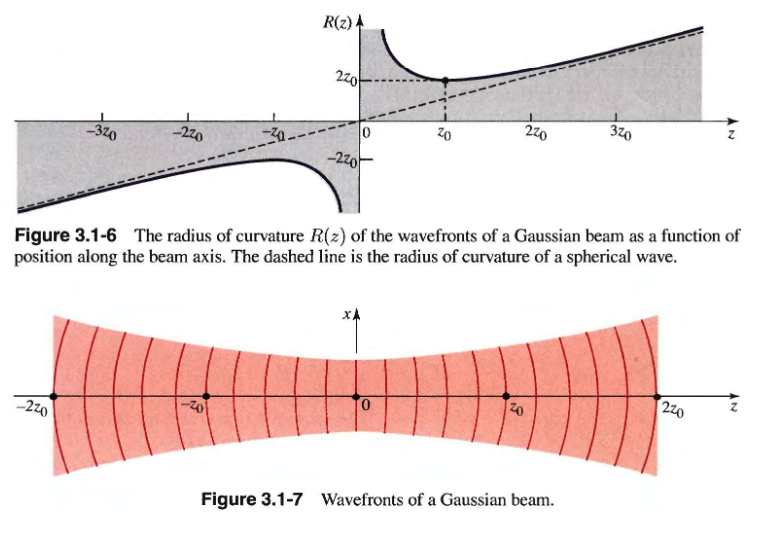
\includegraphics[width=6cm]{gaussian6.png}
		\end{center}
	\end{frame}
	
		\begin{frame}{Wavefronts}

	\end{frame}
	
	
	\begin{frame}{Wavefronts}
	\begin{center}
	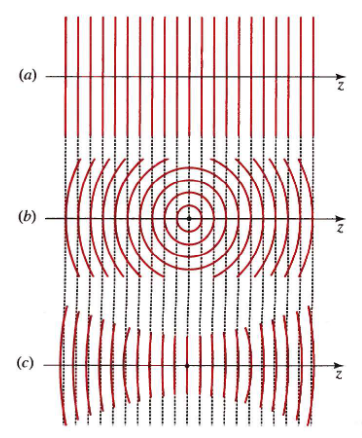
\includegraphics[width=6cm]{gaussian7.png}
\end{center}
	\end{frame}
	
	\begin{frame}{Characterisation of Gaussian Beam}
		
	\end{frame}
	
	\begin{frame}{To Summarize}
		
	\end{frame}
	
	\begin{frame}{Beam Quality}
		
	\end{frame}
	
	\begin{frame}{Beam Quality}
		
	\end{frame}
	
	\begin{frame}{Take-Home Messages}
		
	\end{frame}
	
	\begin{frame}
		\begin{center}
		\LARGE Thank You!!
		\end{center}
	
    \end{frame}
	
	
\end{document}